\section{Beyond Gaussian states}
\label{sec:mixtures}

For one degree of freedom, Gaussian mixtures beat the best Gaussian state: fans of segments through the point of maximal strain by about $5\%$ of the gap, and irregular bundles of needles found by direct optimization by about $8\%$; the gap stays proportional to $\sigma$~\cite{namba2026gap}. In several degrees of freedom the question is how much of this gain survives.

\emph{States.} We use product states: a mixture of $K$ Gaussians in the plane $(v,w)$ of the most stretching mode, combined with one common Gaussian along the configuration direction $a$ of the other mode, the two coupled by a rotation angle $\theta$, and infinitely broad along the momentum direction $b$. The integral along $a$ is then in closed form, so the critical rate is evaluated on a two-dimensional grid; it agrees with a three-dimensional evaluation to $2\times10^{-6}$, and for a single Gaussian with Eq.~\eqref{eq:gaplaw} to $10^{-6}$. The best Gaussian state belongs to this family. Allowing the shape to leave the family afterwards lowered the gap by a further $0.06\%$ ($\varepsilon = 0.1$) and $0.24\%$ ($\varepsilon = 0.3$) of the Gaussian gap, an order of magnitude less than the gain itself.

\emph{Search.} The single pendulum and the coupled pendulums were searched with the same procedure and effort (random hill climbing followed by L-BFGS), from the best one-degree-of-freedom bundles. For the single pendulum the procedure reaches $0.9188\,\sigma$ at $K = 16$, within $0.3\%$ of the best gap found by long searches.

\begin{table}[t]
\caption{Mixtures against the best Gaussian state, $(\kappa - R)/(\kappa - R^*)$, at $\sigma = 10^{-3}$ with the same search for all three systems. Last two columns: the gain $1 - (\kappa-R)/(\kappa-R^*)$ of the coupled system divided by that of the single pendulum.}
\label{tab:mixtures}
\begin{ruledtabular}
\begin{tabular}{llllll}
$K$ & 1 d.o.f. & $\varepsilon = 0.1$ & $\varepsilon = 0.3$ & gain ratio $0.1$ & gain ratio $0.3$ \\
\hline
2 & 0.9795 & 0.9889 & 0.9925 & 0.54 & 0.37 \\
4 & 0.9529 & 0.9728 & 0.9798 & 0.58 & 0.43 \\
8 & 0.9362 & 0.9655 & 0.9751 & 0.54 & 0.39 \\
16 & 0.9196 & 0.9580 & 0.9694 & 0.52 & 0.38 \\
\end{tabular}
\end{ruledtabular}
\end{table}

\begin{observation}[Mixtures gain less in several degrees of freedom]
\label{obs:mixtures}
In two coupled pendulums the gain of mixtures over the best Gaussian state is about $55\%$ ($\varepsilon = 0.1$) and $40\%$ ($\varepsilon = 0.3$) of the gain in one degree of freedom, at every $K$ from $2$ to $16$ (Table~\ref{tab:mixtures}, Fig.~\ref{fig:mixtures}). Almost all of it, $99\%$ for $\varepsilon = 0.1$ and $90\%$ for $\varepsilon = 0.3$ at $K = 8$, comes from mixing inside the plane $(v,w)$ with the law along $a$ kept as in the best Gaussian state. Mixing in the plane raises the cost along $a$ (by $0.03\%$ and $0.5\%$ of the Gaussian gap at $K = 8$), and the optimal mixture partly compensates by widening the law along $a$ by $4$--$7\%$ and reducing $\theta$.
\end{observation}

If mixtures gained only inside the plane and the other directions merely diluted the gain, the ratio would equal the share $f$ of the plane in $\Gamma$, $0.77$ for $\varepsilon = 0.1$ and $0.71$ for $\varepsilon = 0.3$. The observed ratio is smaller: the gain inside the plane is itself smaller than in one degree of freedom, and the cross term along $a$ costs extra. Empirically the ratio is described by $f^{a}$ with $a \approx 2.6$ (fitted; the individual values lie between $2.1$ and $2.9$). As a test, the ratios for $\varepsilon = 1$ and $\varepsilon = -0.3$ were predicted with this law before they were computed, and the predictions were recorded with time and hash (2026-10-13T09:58:04Z; hash beginning \texttt{96300c58}). The predicted gains were within $6\%$ and $3\%$ of the observed ones; for $\varepsilon = -0.3$ the observed value lies inside the predicted range, for $\varepsilon = 1$ just outside it, with a gain slightly larger than predicted. A model that treated the coupled system as a single pendulum with an effective $\beta$, recorded at the same time, overestimated the gain by a factor $1.4$--$1.9$ and is rejected. The exponent $a$ is not derived.

\begin{figure*}[t]
\centering
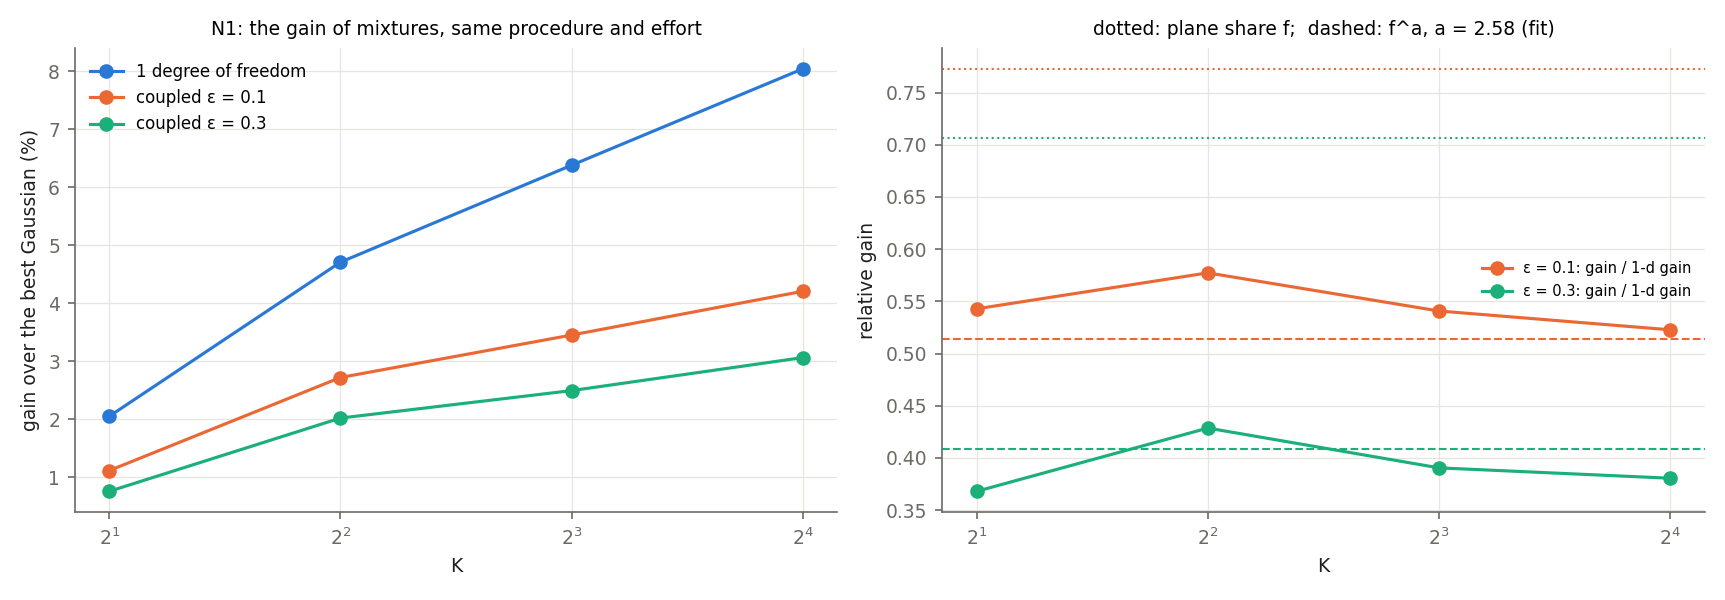
\includegraphics[width=0.95\textwidth]{figures/fig2_mixtures.png}
\caption{Mixtures in one and two degrees of freedom, same search procedure and effort. Left: gain over the best Gaussian state against the number of components $K$. Right: gain of the coupled system divided by that of the single pendulum; dotted lines: share $f$ of the plane $(v,w)$ in $\Gamma$; dashed lines: $f^{a}$ with the fitted $a = 2.58$.}
\label{fig:mixtures}
\end{figure*}
